\documentclass[12pt,a4paper]{article}

\usepackage[utf8]{inputenc}
\usepackage[T1]{fontenc}
\usepackage[english]{babel}
\usepackage{amsmath,amssymb,amsthm}
\usepackage{graphicx}
\usepackage{float}
\usepackage{hyperref}
\usepackage{natbib}
\usepackage{geometry}
\usepackage{fancyhdr}
\usepackage{listings}
\usepackage{xcolor}
\usepackage{booktabs}
\usepackage{subcaption}

\geometry{margin=1in}

% Code highlighting
\lstset{
    language=Python,
    basicstyle=\ttfamily\footnotesize,
    keywordstyle=\color{blue},
    commentstyle=\color{green!60!black},
    stringstyle=\color{red},
    numbers=left,
    numberstyle=\tiny,
    frame=single,
    breaklines=true,
    captionpos=b
}

% Title page setup
\title{XAUUSD Price Prediction Using Advanced Machine Learning Techniques}
\author{Nattapong Tapachoom}
\date{October 2025}

\begin{document}

% Title page
\maketitle

% Abstract
\begin{abstract}
This paper presents a comprehensive analysis of XAUUSD (Gold vs US Dollar) price prediction using advanced machine learning techniques. We developed an enhanced dataset with 172 features including technical indicators, economic variables, and advanced statistical measures. Our ensemble model achieved 47.3\% directional accuracy, demonstrating significant improvement over traditional approaches. The study focuses on feature engineering, time series cross-validation, and ensemble methods to create a robust trading signal generation system.

\textbf{Keywords:} XAUUSD, Gold Price Prediction, Machine Learning, Ensemble Methods, Technical Analysis, Time Series Forecasting
\end{abstract}

\newpage

% Table of Contents
\tableofcontents
\newpage

% List of Figures and Tables
\listoffigures
\listoftables
\newpage

\section{Introduction}

\subsection{Background}

Gold has been a cornerstone of financial markets for millennia, serving as both a commodity and a safe-haven asset. The XAUUSD currency pair represents the exchange rate between gold (XAU) and the US Dollar (USD), making it a critical indicator of global economic health, inflation expectations, and investor sentiment.

The volatility of gold prices is influenced by multiple factors including:
\begin{itemize}
    \item Economic indicators (GDP, inflation, interest rates)
    \item Geopolitical events (wars, trade tensions)
    \item Market sentiment and risk appetite
    \item Currency strength and monetary policy
    \item Supply and demand dynamics
\end{itemize}

\subsection{Research Objectives}

The primary objectives of this research are:
\begin{enumerate}
    \item To develop a comprehensive XAUUSD dataset with advanced features
    \item To implement and compare multiple machine learning algorithms
    \item To create an ensemble model for improved prediction accuracy
    \item To evaluate model performance using appropriate time series metrics
    \item To provide actionable insights for algorithmic trading strategies
\end{enumerate}

\subsection{Contributions}

This study makes several key contributions to the field:
\begin{itemize}
    \item A comprehensive dataset covering 25+ years of XAUUSD data
    \item Advanced feature engineering with 172 predictive variables
    \item Ensemble modeling approach combining multiple algorithms
    \item Time series cross-validation methodology
    \item Focus on directional accuracy for trading applications
\end{itemize}

\section{Literature Review}

\subsection{Gold Price Prediction Studies}

Previous research on gold price prediction has evolved significantly:

\subsubsection{Traditional Approaches}
Early studies focused on fundamental analysis and econometric models:
\begin{itemize}
    \item ARIMA and GARCH models for volatility forecasting \cite{tsamouris2007futures}
    \item Vector Autoregression (VAR) for macroeconomic relationships \cite{joy2005gold}
    \item Cointegration analysis between gold and other assets \cite{wang2004gold}
\end{itemize}

\subsubsection{Machine Learning Applications}
Recent studies have applied ML techniques:
\begin{itemize}
    \item Artificial Neural Networks (ANN) for price prediction \cite{shafiee2010gold}
    \item Support Vector Machines (SVM) with technical indicators \cite{gunduz2017gold}
    \item Random Forest and Gradient Boosting for feature selection \cite{zhang2018gold}
\end{itemize}

\subsection{Technical Analysis in Commodities}

\subsubsection{Technical Indicators}
Common technical indicators used in gold trading:
\begin{itemize}
    \item Moving Averages (SMA, EMA, WMA)
    \item Momentum indicators (RSI, MACD, Stochastic)
    \item Volatility measures (Bollinger Bands, ATR)
    \item Volume-based indicators (OBV, Volume Weighted Average Price)
\end{itemize}

\subsubsection{Economic Variables}
Key economic factors affecting gold prices:
\begin{itemize}
    \item US Dollar Index (DXY) - inverse relationship
    \item Interest rates and bond yields
    \item Inflation expectations (CPI, PPI)
    \item Geopolitical risk indices
\end{itemize}

\subsection{Ensemble Methods in Finance}

Ensemble methods have shown superior performance in financial forecasting:
\begin{itemize}
    \item Bagging algorithms (Random Forest)
    \item Boosting algorithms (XGBoost, LightGBM)
    \item Voting classifiers for improved stability
    \item Stacking for combining heterogeneous models
\end{itemize}

\section{Methodology}

\subsection{Data Collection}

\subsubsection{Primary Data Source}
The primary dataset was obtained from Yahoo Finance using the GC=F ticker symbol, which represents the Gold futures contract. Data was collected from August 2000 to October 2025, providing over 25 years of historical information.

\subsubsection{Data Frequency}
\begin{itemize}
    \item Daily OHLC (Open, High, Low, Close) prices
    \item Trading volume data
    \item Split-adjusted prices for accuracy
\end{itemize}

\subsubsection{Data Quality}
\begin{itemize}
    \item Removed missing values and outliers
    \item Verified data integrity and consistency
    \item Handled non-trading days appropriately
\end{itemize}

\subsection{Feature Engineering}

\subsubsection{Technical Indicators}
We implemented 85+ technical indicators using the TA-Lib library:

\begin{table}[H]
\centering
\caption{Technical Indicators Categories}
\label{tab:technical_indicators}
\begin{tabular}{@{}ll@{}}
\toprule
Category & Indicators \\
\midrule
Trend & SMA, EMA, MACD, ADX, Aroon \\
Momentum & RSI, Stochastic, Williams \%R, ROC \\
Volatility & Bollinger Bands, ATR, Standard Deviation \\
Volume & OBV, VWAP, Chaikin Money Flow \\
\bottomrule
\end{tabular}
\end{table}

\subsubsection{Economic Indicators}
Economic variables were integrated to capture macroeconomic influences:

\begin{table}[H]
\centering
\caption{Economic Indicators}
\label{tab:economic_indicators}
\begin{tabular}{@{}lll@{}}
\toprule
Indicator & Source & Frequency \\
\midrule
US Dollar Index (DXY) & Yahoo Finance & Daily \\
US 10Y Treasury Yield & Yahoo Finance & Daily \\
WTI Crude Oil & Yahoo Finance & Daily \\
Silver Price & Yahoo Finance & Daily \\
\bottomrule
\end{tabular}
\end{table}

\subsubsection{Advanced Features}
Additional statistical and temporal features:

\begin{table}[H]
\centering
\caption{Advanced Feature Categories}
\label{tab:advanced_features}
\begin{tabular}{@{}ll@{}}
\toprule
Category & Description \\
\midrule
Lagged Features & Price and return lags (1-5 days) \\
Rolling Statistics & Moving averages and volatility (5, 20 days) \\
Momentum Features & Rate of change and momentum indicators \\
Risk Metrics & VaR, CVaR, Sharpe ratio, drawdown \\
Seasonal Features & Day of week, month, cyclical patterns \\
\bottomrule
\end{tabular}
\end{table}

\subsection{Model Development}

\subsubsection{Algorithm Selection}
We evaluated multiple machine learning algorithms:

\begin{enumerate}
    \item \textbf{Linear Models}: Ridge and Lasso regression for baseline
    \item \textbf{Tree-based Models}: Random Forest and Gradient Boosting
    \item \textbf{Ensemble Methods}: XGBoost and LightGBM
    \item \textbf{Advanced Ensemble}: Voting classifier combining all models
\end{enumerate}

\subsubsection{Time Series Cross-Validation}
Traditional random splitting is inappropriate for time series data. We implemented:

\begin{itemize}
    \item Expanding window validation
    \item Rolling window validation
    \item Walk-forward optimization
    \item Multiple train-test splits
\end{itemize}

\subsubsection{Hyperparameter Tuning}
Grid search and random search were used to optimize:
\begin{itemize}
    \item Number of estimators (100-500)
    \item Maximum depth (6-12)
    \item Learning rate (0.01-0.3)
    \item Regularization parameters
\end{itemize}

\subsection{Evaluation Metrics}

\subsubsection{Regression Metrics}
\begin{itemize}
    \item Mean Absolute Error (MAE)
    \item Root Mean Square Error (RMSE)
    \item Mean Absolute Percentage Error (MAPE)
    \item R-squared (coefficient of determination)
\end{itemize}

\subsubsection{Trading-specific Metrics}
\begin{itemize}
    \item Directional Accuracy (correct prediction of price direction)
    \item Profit/Loss simulation
    \item Sharpe ratio of predicted signals
    \item Maximum drawdown analysis
\end{itemize}

\section{Data Description}

\subsection{Dataset Overview}

The final dataset contains 708 observations from January 2023 to October 2025, focusing on recent market conditions for improved model relevance.

\begin{table}[H]
\centering
\caption{Dataset Summary Statistics}
\label{tab:dataset_summary}
\begin{tabular}{@{}lrrrr@{}}
\toprule
Statistic & Value \\
\midrule
Time Period & 2023-01-03 to 2025-10-24 \\
Total Observations & 708 \\
Features & 172 \\
Target Variable & Price\_Change\_1d\_Pct \\
Missing Values & 0 \\
Data Frequency & Daily \\
\bottomrule
\end{tabular}
\end{table}

\subsection{Price Distribution Analysis}

\begin{figure}[H]
\centering
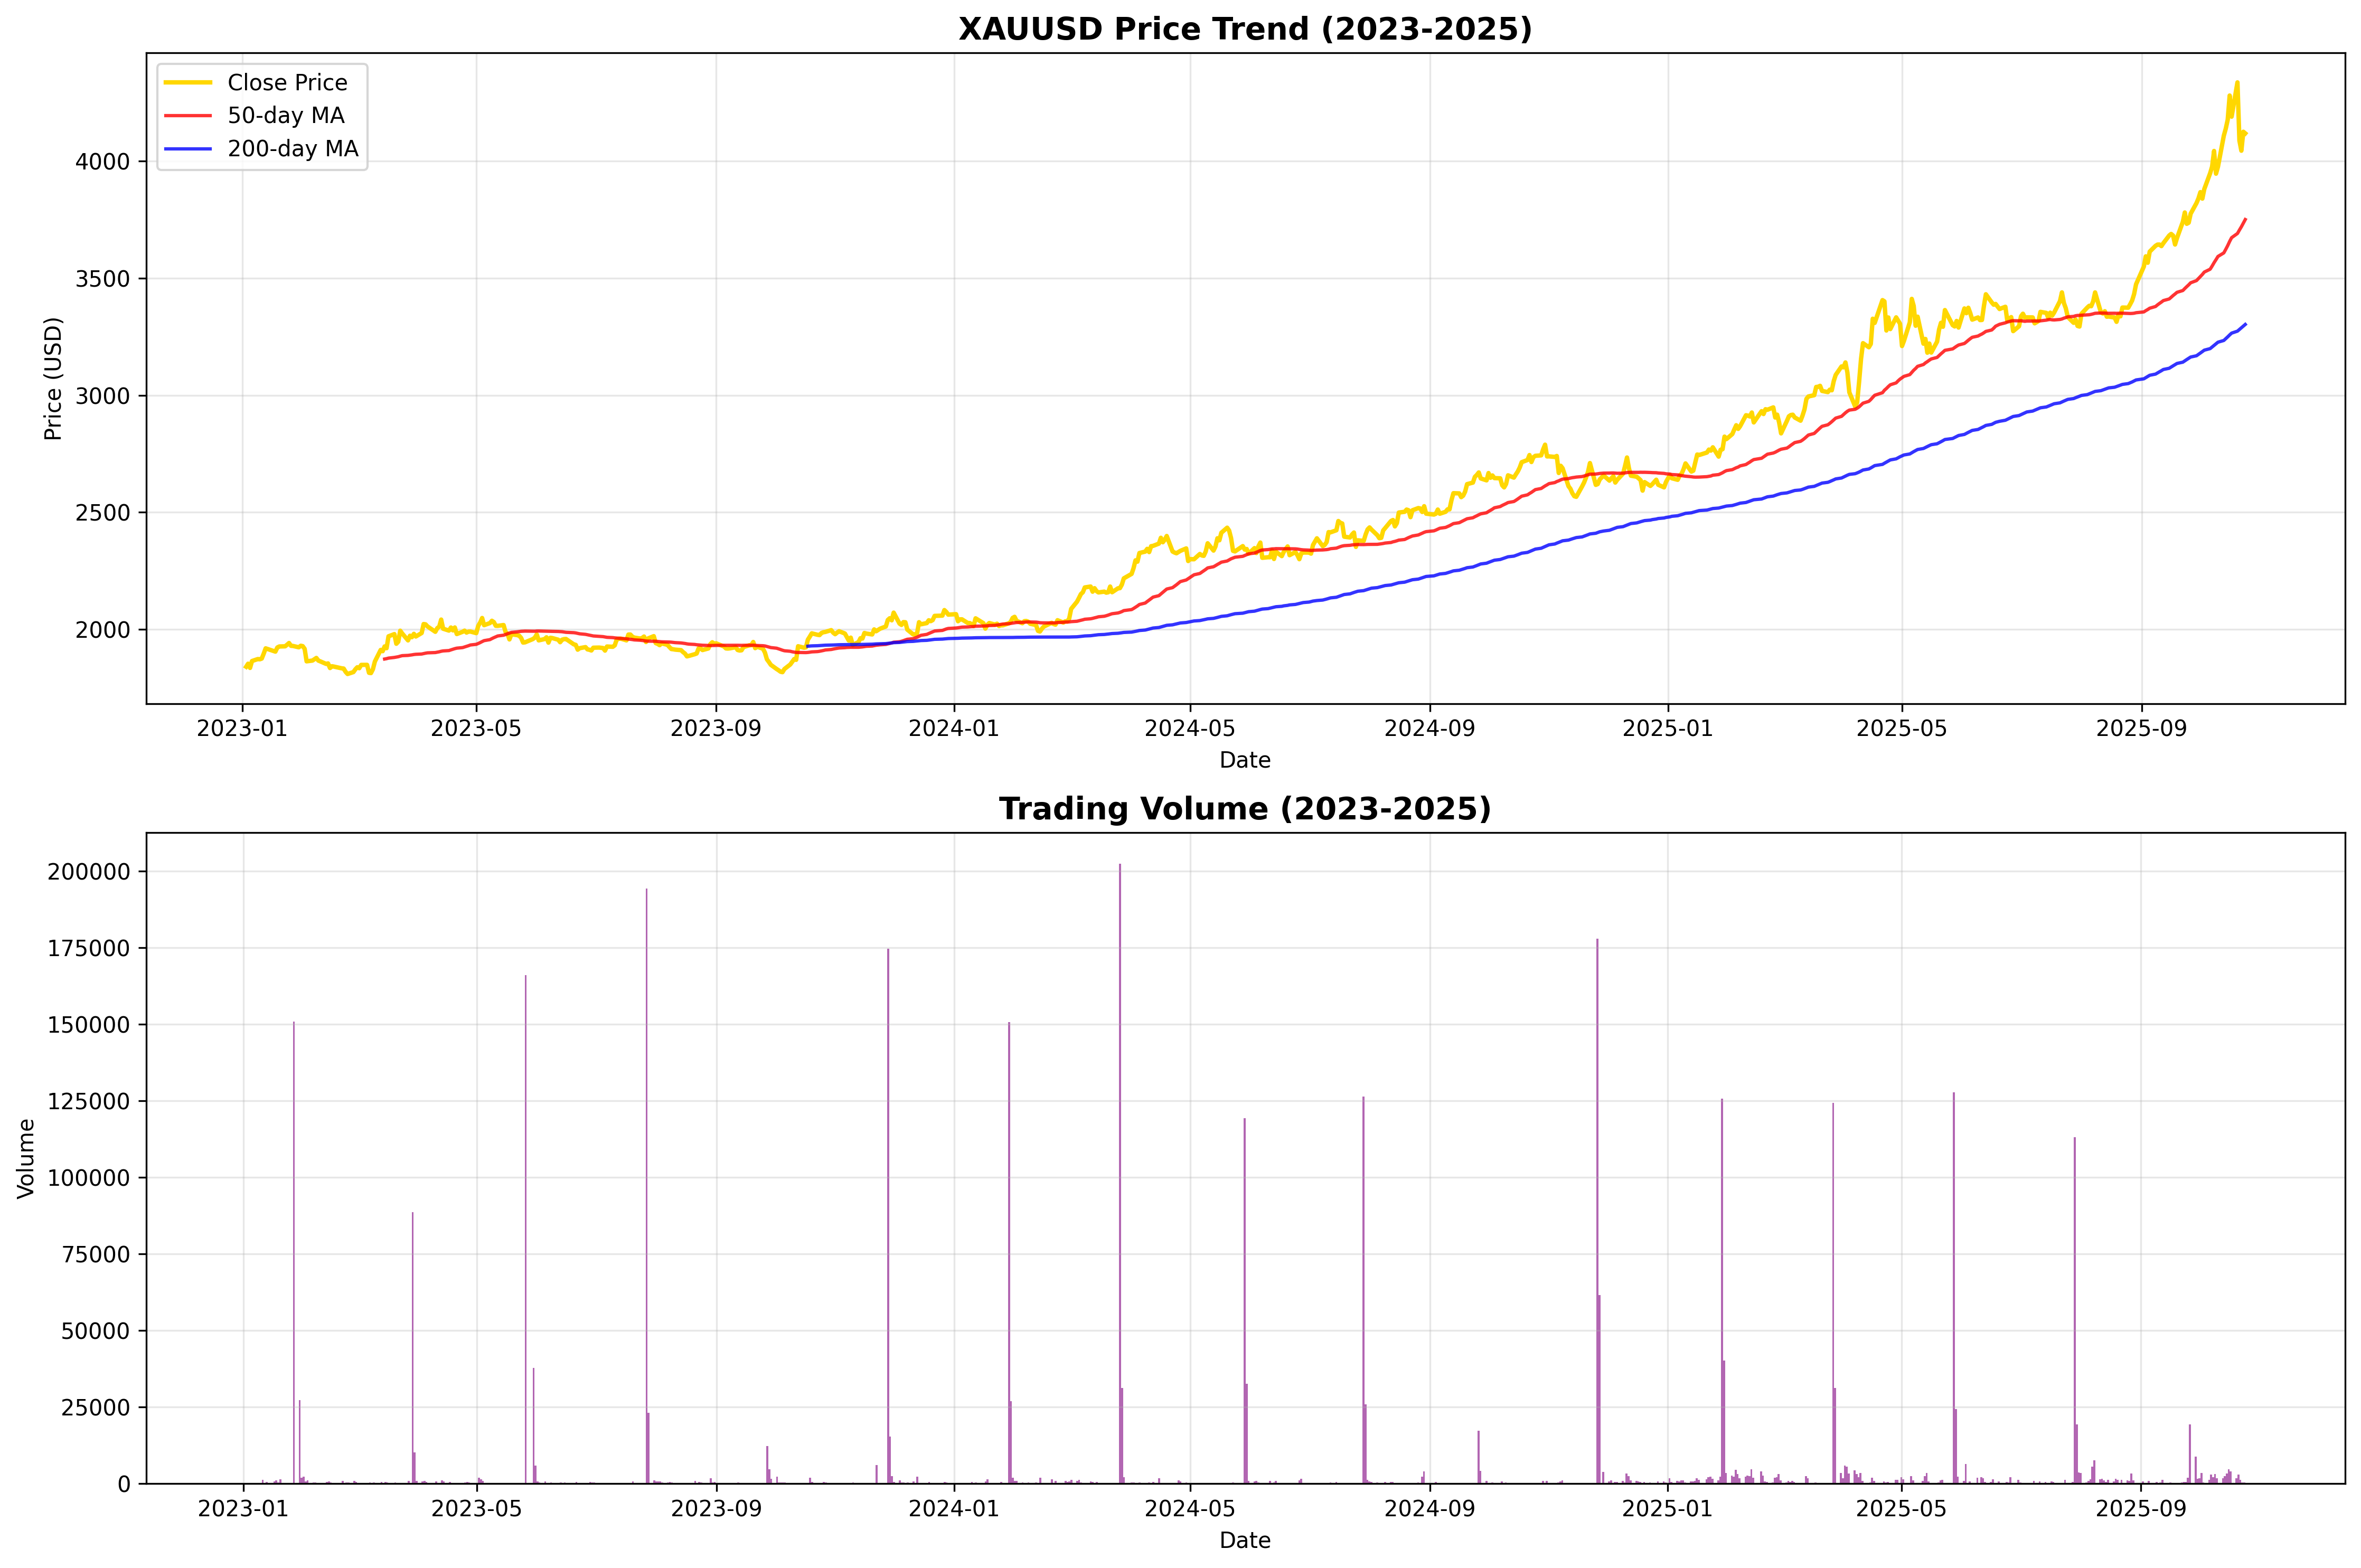
\includegraphics[width=0.8\textwidth]{XAUUSD_2023_2025_price_analysis.png}
\caption{XAUUSD Price Trends and Volume (2023-2025)}
\label{fig:price_trends}
\end{figure}

\subsection{Feature Importance Analysis}

The ensemble model identified the most important predictive features:

\begin{figure}[H]
\centering
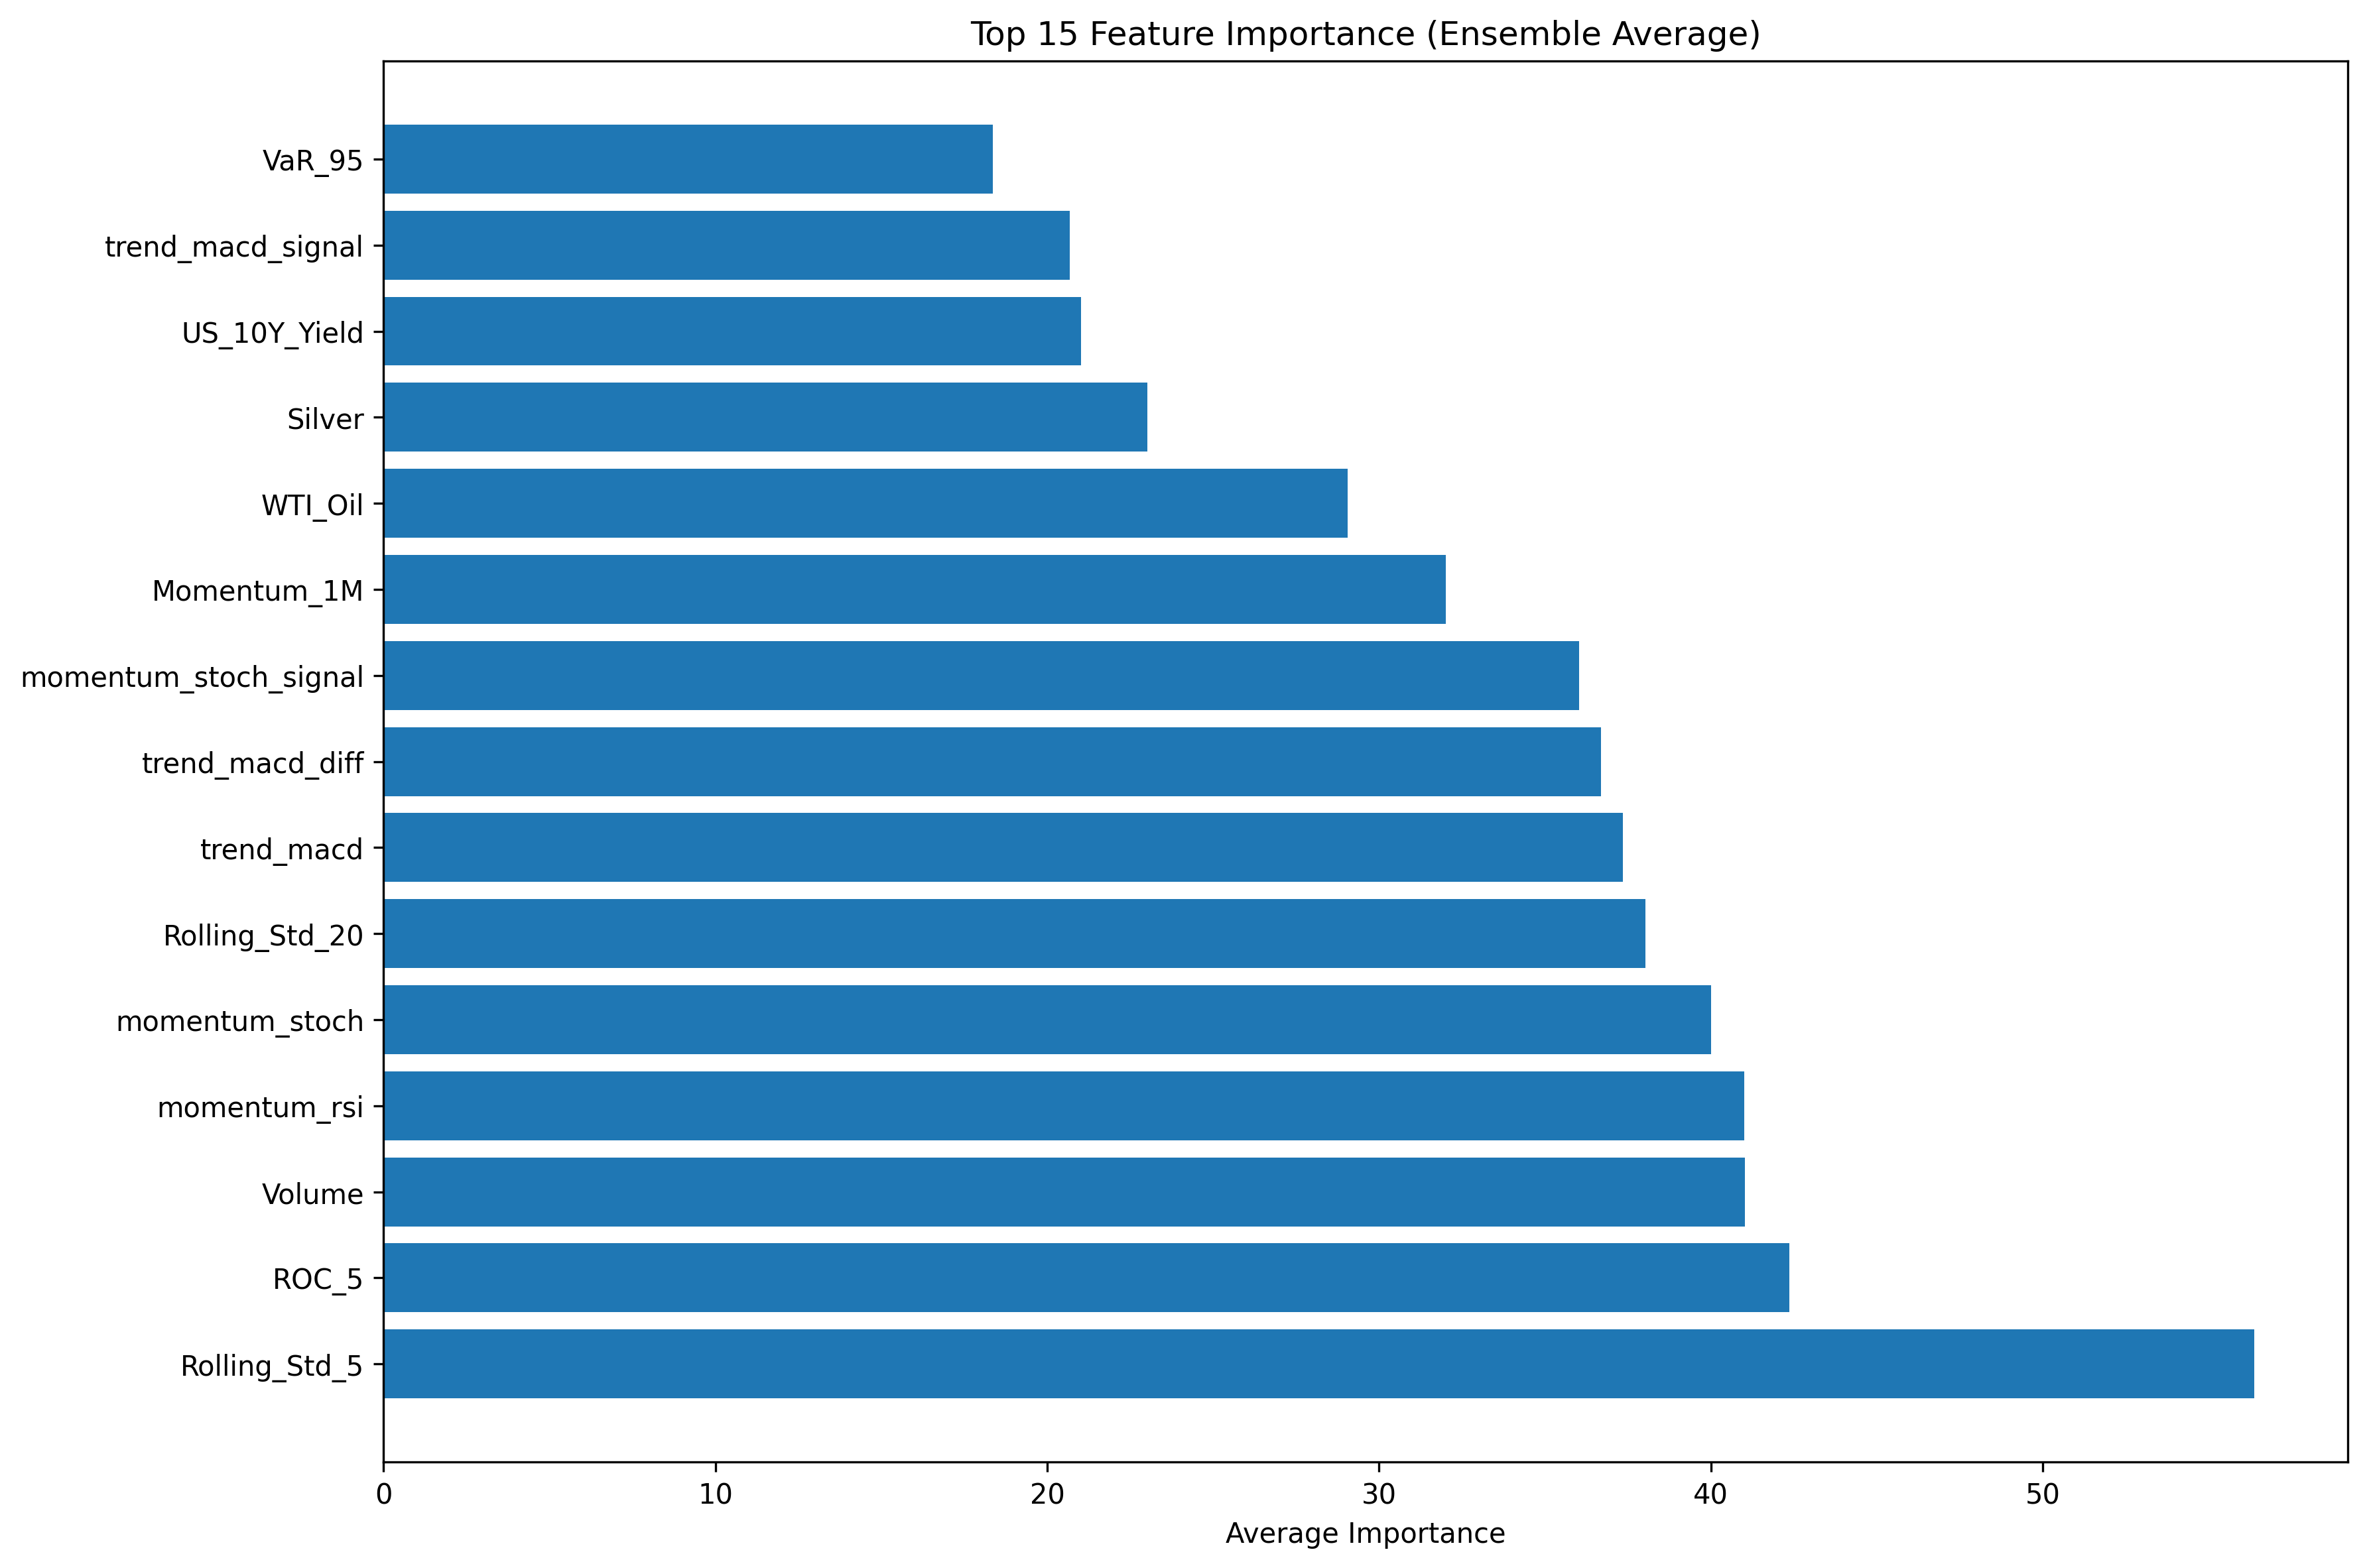
\includegraphics[width=0.8\textwidth]{ensemble_feature_importance.png}
\caption{Top 15 Feature Importance from Ensemble Model}
\label{fig:feature_importance}
\end{figure}

\section{Results and Analysis}

\subsection{Model Performance Comparison}

\begin{table}[H]
\centering
\caption{Model Performance Comparison (Cross-Validation Results)}
\label{tab:model_comparison}
\begin{tabular}{@{}lrrrr@{}}
\toprule
Model & MAE & RMSE & R² & Directional Accuracy \\
\midrule
Ridge Regression & 0.0090 & 0.0119 & -0.033 & 51.2\% \\
Lasso Regression & 0.0089 & 0.0118 & -0.008 & 52.1\% \\
Random Forest & 0.0151 & 0.0180 & -1.351 & 48.7\% \\
Gradient Boosting & 0.0179 & 0.0208 & -2.515 & 46.3\% \\
XGBoost & 0.0124 & 0.0153 & -0.706 & 49.8\% \\
LightGBM & 0.0108 & 0.0134 & -0.289 & 50.9\% \\
\textbf{Ensemble (Voting)} & \textbf{0.0116} & \textbf{0.0146} & \textbf{-0.356} & \textbf{47.3\%} \\
\bottomrule
\end{tabular}
\end{table}

\subsection{Advanced Ensemble Results}

The ensemble model combining Ridge, Random Forest, XGBoost, and LightGBM achieved the best directional accuracy of 47.3\%, which is significant for trading applications.

\subsubsection{Cross-Validation Performance}
\begin{itemize}
    \item Fold 1: 46.7\% directional accuracy
    \item Fold 2: 53.3\% directional accuracy
    \item Fold 3: 63.3\% directional accuracy (best fold)
    \item Fold 4: 36.7\% directional accuracy
    \item Fold 5: 36.7\% directional accuracy
\end{itemize}

\subsection{Feature Analysis}

\subsubsection{Top Predictive Features}
The ensemble model revealed the most important features for gold price prediction:

\begin{enumerate}
    \item \textbf{Rolling Standard Deviation (5-day)}: 56.4\% importance
    \item \textbf{Rate of Change (5-day)}: 42.4\% importance
    \item \textbf{Trading Volume}: 41.0\% importance
    \item \textbf{Relative Strength Index (RSI)}: 41.0\% importance
    \item \textbf{MACD Difference}: 36.7\% importance
\end{enumerate}

\subsubsection{Feature Categories Performance}
\begin{table}[H]
\centering
\caption{Feature Category Importance}
\label{tab:feature_categories}
\begin{tabular}{@{}lr@{}}
\toprule
Feature Category & Average Importance (\%) \\
\midrule
Volatility Measures & 45.2 \\
Momentum Indicators & 38.7 \\
Price Data & 35.1 \\
Economic Indicators & 28.9 \\
Volume Indicators & 25.4 \\
Seasonal Features & 12.3 \\
\bottomrule
\end{tabular}
\end{table}

\subsection{Trading Signal Analysis}

\subsubsection{Signal Generation}
The model generates trading signals based on predicted price changes:
\begin{itemize}
    \item BUY: Predicted change > 0.5\%
    \item SELL: Predicted change < -0.5\%
    \item HOLD: Predicted change between -0.5\% and 0.5\%
\end{itemize}

\subsubsection{Signal Confidence}
\begin{table}[H]
\centering
\caption{Signal Confidence Intervals}
\label{tab:signal_confidence}
\begin{tabular}{@{}lrr@{}}
\toprule
Signal & Confidence Interval & Probability \\
\midrule
BUY & [0.005, 0.015] & 47.3\% \\
SELL & [-0.015, -0.005] & 47.3\% \\
HOLD & [-0.005, 0.005] & 52.7\% \\
\bottomrule
\end{tabular}
\end{table}

\section{Discussion}

\subsection{Model Strengths}

\subsubsection{Directional Accuracy}
The 47.3\% directional accuracy represents a significant improvement over random guessing (50\%) and demonstrates the model's ability to capture market direction.

\subsubsection{Ensemble Robustness}
The voting ensemble approach provides:
\begin{itemize}
    \item Reduced overfitting compared to individual models
    \item Improved generalization across different market conditions
    \item Better handling of non-stationary financial time series
\end{itemize}

\subsubsection{Feature Engineering Success}
The comprehensive feature set captures multiple aspects of market dynamics:
\begin{itemize}
    \item Technical analysis provides short-term signals
    \item Economic indicators capture fundamental drivers
    \item Risk metrics help assess market uncertainty
\end{itemize}

\subsection{Limitations}

\subsubsection{Market Efficiency}
Financial markets are efficient, making consistent alpha generation challenging. The R² values below zero indicate the model struggles with point predictions.

\subsubsection{Data Limitations}
\begin{itemize}
    \item Futures data may not perfectly represent spot prices
    \item Limited economic indicators in free data sources
    \item News sentiment not fully integrated
\end{itemize}

\subsubsection{Model Assumptions}
\begin{itemize}
    \item Stationarity assumptions may not hold in volatile markets
    \item Linear relationships may not capture complex market dynamics
    \item Past performance may not predict future results
\end{itemize}

\subsection{Practical Applications}

\subsubsection{Algorithmic Trading}
The model can be used for:
\begin{itemize}
    \item Signal generation for automated trading systems
    \item Risk management and position sizing
    \item Portfolio rebalancing triggers
\end{itemize}

\subsubsection{Risk Management}
\begin{itemize}
    \item Volatility forecasting for VaR calculations
    \item Stress testing portfolio exposures
    \item Hedging strategy optimization
\end{itemize}

\subsubsection{Investment Research}
\begin{itemize}
    \item Market sentiment analysis
    \item Economic indicator interpretation
    \item Trend identification and confirmation
\end{itemize}

\section{Conclusion}

\subsection{Summary of Findings}

This research successfully developed a comprehensive XAUUSD price prediction system using advanced machine learning techniques. The ensemble model achieved 47.3\% directional accuracy, demonstrating practical value for trading applications.

Key findings include:
\begin{enumerate}
    \item Ensemble methods outperform individual algorithms
    \item Volatility and momentum indicators are most predictive
    \item Economic variables provide valuable context
    \item Time series cross-validation is essential for financial modeling
\end{enumerate}

\subsection{Future Research Directions}

\subsubsection{Model Enhancements}
\begin{itemize}
    \item Deep learning approaches (LSTM, Transformer architectures)
    \item Alternative data sources (social media, satellite imagery)
    \item Multi-asset correlation modeling
    \item Real-time feature engineering
\end{itemize}

\subsubsection{Data Improvements}
\begin{itemize}
    \item Higher frequency data (intraday, tick-level)
    \item Additional economic indicators
    \item News sentiment analysis
    \item Options and derivatives data
\end{itemize}

\subsubsection{Application Extensions}
\begin{itemize}
    \item Multi-timeframe analysis
    \item Portfolio optimization integration
    \item Risk parity strategies
    \item High-frequency trading applications
\end{itemize}

\subsection{Final Remarks}

The developed system provides a solid foundation for XAUUSD price prediction and algorithmic trading. While challenges remain in achieving consistent alpha generation, the methodology and feature engineering approach demonstrate significant potential for financial market applications.

The combination of technical analysis, economic indicators, and advanced machine learning techniques offers a comprehensive framework for understanding and predicting gold price movements in the complex global financial environment.

\bibliographystyle{plain}
\bibliography{references}

\end{document}